%%%%%%%%%%%%%%%%%%%%%%%%%%%%%%%%%%%%%%%%%%%%%%%%%%%%%%%%%%%%%%%%
%
%  Template for homework of Introduction to Machine Learning.
%
%  Fill in your name, lecture number, lecture date and body
%  of homework as indicated below.
%
%%%%%%%%%%%%%%%%%%%%%%%%%%%%%%%%%%%%%%%%%%%%%%%%%%%%%%%%%%%%%%%%


\documentclass[11pt,letter,notitlepage]{article}

\usepackage[left=2cm, right=2cm, lines=45, top=0.8in, bottom=0.7in]{geometry}

\usepackage{fancyhdr}
\usepackage{fancybox}
\usepackage{graphicx}
\usepackage{pdfpages} 
\usepackage{enumitem}
\usepackage{algorithm}
\usepackage{algorithmic}

\usepackage{epstopdf}
\usepackage{subfigure}
\usepackage{threeparttable}


\renewcommand{\headrulewidth}{1.5pt}
\renewcommand{\footrulewidth}{1.5pt}
\newcommand\Loadedframemethod{TikZ}
\usepackage[framemethod=\Loadedframemethod]{mdframed}

\usepackage{amssymb,amsmath}
\usepackage{amsthm}
\usepackage{thmtools}

\setlength{\topmargin}{0pt}
\setlength{\textheight}{9in}
\setlength{\headheight}{0pt}

\setlength{\oddsidemargin}{0.25in}
\setlength{\textwidth}{6in}

%%%%%%%%%%%%%%%%%%%%%%%%
%%%%%% Define math operator %%%%%
%%%%%%%%%%%%%%%%%%%%%%%%
\DeclareMathOperator*{\argmin}{\bf argmin}
\DeclareMathOperator*{\argmax}{\bf argmax}
\DeclareMathOperator*{\relint}{\bf relint\,}
\DeclareMathOperator*{\dom}{\bf dom\,}
\DeclareMathOperator*{\intp}{\bf int\,}
%%%%%%%%%%%%%%%%%%%%%%%


\setlength{\topmargin}{0pt}
\setlength{\textheight}{9in}
\setlength{\headheight}{0pt}

\setlength{\oddsidemargin}{0.25in}
\setlength{\textwidth}{6in}
\pagestyle{fancy}
%%%%%%%%%%%%%%%%%%%%%%%%
%% Define the Exercise environment %%
%%%%%%%%%%%%%%%%%%%%%%%%
\mdtheorem[
topline=false,
rightline=false,
leftline=false,
bottomline=false,
leftmargin=-10,
rightmargin=-10
]{exercise}{\textbf{Exercise}}
%%%%%%%%%%%%%%%%%%%%%%%
%% End of the Exercise environment %%
%%%%%%%%%%%%%%%%%%%%%%%


%%%%%%%%%%%%%%%%%%%%%%%%
%% Define the Problem environment %%
%%%%%%%%%%%%%%%%%%%%%%%%
\mdtheorem[
topline=false,
rightline=false,
leftline=false,
bottomline=false,
leftmargin=-10,
rightmargin=-10
]{problem}{\textbf{Problem}}
%%%%%%%%%%%%%%%%%%%%%%%
%% End of the Exercise environment %%
%%%%%%%%%%%%%%%%%%%%%%%

%%%%%%%%%%%%%%%%%%%%%%%
%% Define the Solution Environment %%
%%%%%%%%%%%%%%%%%%%%%%%
\declaretheoremstyle
[
spaceabove=0pt, 
spacebelow=0pt, 
headfont=\normalfont\bfseries,
notefont=\mdseries, 
notebraces={(}{)}, 
headpunct={:\quad}, 
headindent={},
postheadspace={ }, 
postheadspace=4pt, 
bodyfont=\normalfont, 
qed=$\blacksquare$,
preheadhook={\begin{mdframed}[style=myframedstyle]\end{mdframed}},
	postfoothook={},
]{mystyle}

\declaretheorem[style=mystyle,title=Solution,numbered=no]{solution}
\mdfdefinestyle{myframedstyle}{%
	topline=false,
	rightline=false,
	leftline=false,
	bottomline=false,
	skipabove=-6ex,
	leftmargin=-10,
	rightmargin=-10}
%%%%%%%%%%%%%%%%%%%%%%%
%% End of the Solution environment %%
%%%%%%%%%%%%%%%%%%%%%%%

%% Homework info.
\newcommand{\posted}{\text{December 24, 2024}}       			%%% FILL IN POST DATE HERE
\newcommand{\due}{\text{January 2, 2024}} 			%%% FILL IN Due DATE HERE
\newcommand{\hwno}{\text{7}} 		           			%%% FILL IN LECTURE NUMBER HERE


\newcommand{\expect}[1]{\text{E} [#1]}
\newcommand{\var}[1]{\text{Var} [#1]}

%%%%%%%%%%%%%%%%%%%%
%% Put your information here %%
%%%%%%%%%%%%%%%%%%%
\newcommand{\name}{\text{San Zhang}}  	          			%%% FILL IN YOUR NAME HERE
\newcommand{\id}{\text{PBXXXXXXXX}}		       			%%% FILL IN YOUR ID HERE
%%%%%%%%%%%%%%%%%%%%
%% End of the student's info %%
%%%%%%%%%%%%%%%%%%%



\chead{\textbf{
		Homework \hwno
}}


\begin{document}
\vspace*{-4\baselineskip}
\thispagestyle{empty}


\begin{center}
{\bf\large Introduction to Machine Learning}\\
{Fall 2024}\\
University of Science and Technology of China
\end{center}

\noindent
Lecturer: Jie Wang  			 %%% FILL IN LECTURER HERE
\hfill
Homework \hwno             			
\\
Posted: \posted
\hfill
Due: \due

\noindent
\rule{\textwidth}{2pt}

\medskip





%%%%%%%%%%%%%%%%%%%%%%%%%%%%%%%%%%%%%%%%%%%%%%%%%%%%%%%%%%%%%%%%
%% BODY OF HOMEWORK GOES HERE
%%%%%%%%%%%%%%%%%%%%%%%%%%%%%%%%%%%%%%%%%%%%%%%%%%%%%%%%%%%%%%%%

\textbf{Notice, }to get the full credits, please present your solutions step by step.

\begin{exercise}[Singular Value Decomposition]
    Let $\mathbf{A}\in\mathbb{R}^{m\times n}$, $\operatorname{rank} \mathbf{A}=r$. The SVD of $\mathbf{A}$ is $\mathbf{A}=\mathbf{U\Sigma V}^{\top}$, where $\mathbf{U}\in \mathbb{R}^{m\times m},\mathbf{\Sigma}\in\mathbb{R}^{m\times n}, \mathbf{V}\in\mathbb{R}^{n\times n}$, and we sort the diagonal entries of $\mathbf{\Sigma}$ in the descending order $\sigma_1\geq\sigma_2\geq\ldots\geq\sigma_r>0$. Denote
    \begin{align*}
        &\mathbf{U_1}=(\mathbf{u}_{1},\mathbf{u}_{2},\ldots,\mathbf{u}_{r}),\  \mathbf{U_2}=(\mathbf{u}_{r+1},\ldots,\mathbf{u}_{m}),\\
        &\mathbf{V_1}=(\mathbf{v}_{1},\mathbf{v}_{2},\ldots,\mathbf{v}_{r}),\  \mathbf{V_2}=(\mathbf{v}_{r+1},\ldots,\mathbf{v}_{n}).
    \end{align*}
    The column space of $\mathbf{A}$ is the set 
    \begin{align*}
        \mathcal{C}(\mathbf{A}) = \{\mathbf{y}\in\mathbb{R}^m: \mathbf{y}=\mathbf{A}\mathbf{x}, \mathbf{x}\in\mathbb{R}^n\}.
    \end{align*}
    The null space of $\mathbf{A}$ is the set
    \begin{align*}
        \mathcal{N}(\mathbf{A})=\{\mathbf{y}\in\mathbb{R}^n: \mathbf{A}\mathbf{y}=\mathbf{0}\}.
    \end{align*}
    
    \begin{enumerate}
        \item Show that 
            \begin{enumerate}
                \item $P_{\mathcal{C}(\mathbf{A})}(\mathbf{x})=\mathbf{U_1U_1}^{\top}\mathbf{x}$;
                \item $P_{\mathcal{N}(\mathbf{A})}(\mathbf{x})=\mathbf{V_2V_2}^{\top}\mathbf{x}$;
                \item $P_{\mathcal{C}(\mathbf{A}^{\top})}(\mathbf{x})=\mathbf{V_1V_1}^{\top}\mathbf{x}$;
                \item $P_{\mathcal{N}(\mathbf{A}^{\top})}(\mathbf{x})=\mathbf{U_2U_2}^{\top}\mathbf{x}$.
            \end{enumerate}
            
        \item The Frobenius norm of $\mathbf{A}$ is
            \begin{align*}
                \|\mathbf{A}\|_F=\sqrt{\sum_{i=1}^m\sum_{j=1}^na_{i,j}^2}.
            \end{align*}
            \begin{enumerate}
                \item Show that $\|\mathbf{A}\|_F^2=\operatorname{tr}(\mathbf{A}^{\top}\mathbf{A})$.
                
                \item Let $\mathbf{B}\in\mathbb{R}^{m\times n}$. Suppose that $\mathcal{C}(\mathbf{A})\bot\mathcal{C}(\mathbf{B})$, that is, 
                \begin{align*}
                    \langle\mathbf{a},\mathbf{b}\rangle=0,\,\forall\,\mathbf{a}\in\mathcal{C}(\mathbf{A}),\,\mathbf{b}\in\mathcal{C}(\mathbf{B}).
                \end{align*}
                Show that
                \begin{align*}
                    \|\mathbf{A}+\mathbf{B}\|_F^2=\|\mathbf{A}\|_F^2+\|\mathbf{B}\|_F^2.
                \end{align*}
            \end{enumerate}
            
        
    \end{enumerate}
\end{exercise}

\begin{solution}${}$
\end{solution}


\newpage

\begin{exercise}[Principle Component Analysis]
    Suppose that we have a set of data instances $\{\mathbf{x}_i\}_{i=1}^n\subset\mathbb{R}^d$. Let $\widetilde{\mathbf{X}}\in\mathbb{R}^{d\times n}$ be the matrix whose $i^{th}$ column is $\mathbf{x}_i-\Bar{\mathbf{x}}$, where $\Bar{\mathbf{x}}$ is the sample mean, and $\mathbf{S}$ be the sample variance matrix.

    \begin{enumerate}
        \item For $\mathbf{G}\in\mathbb{R}^{d\times K}$, let us define
        \begin{align}\label{eqn:obj-PCA}
            f(\mathbf{G}) = \operatorname{tr}(\mathbf{G}^{\top}\mathbf{SG}).
        \end{align}
        Show that $f(\mathbf{GQ})=f(\mathbf{G})$ for any orthogonal matrix $\mathbf{Q}\in\mathbb{R}^{K\times K}$.
        
        \item Please find $\mathbf{g}_1$ defined as follows by the Lagrange multiplier method.
            \begin{align}\label{eqn:PC1}
                \mathbf{g}_1:=\argmax_{\mathbf{g}\in\mathbb{R}^d}\{f(\mathbf{g}):\|\mathbf{g}\|_2=1\},
            \end{align}
            where $f$ is defined by (\ref{eqn:obj-PCA}). Notice that, the vector $\mathbf{g}_1$ is the first principal component vector of the data.
            
        \item Please find $\mathbf{g}_2$ defined as follows by the Lagrange multiplier method.
            \begin{align*}
                \mathbf{g}_2:=\argmax_{\mathbf{g}\in\mathbb{R}^d}\{f(\mathbf{g}):\|\mathbf{g}\|_2=1,\langle\mathbf{g},\mathbf{g}_1\rangle=0\},
            \end{align*}
            where $\mathbf{g}_1$ is given by (\ref{eqn:PC1}). Similar to $\mathbf{g}_1$, the vector $\mathbf{g}_2$ is the second principal component vector of the data.
            
        \item Please derive the first $K$ principal component vectors by repeating the above process.
        
        \item What is $f(\mathbf{g}_k)$, $k=1,\ldots,K$? What about their meaning?
        
    \end{enumerate}
\end{exercise}
\begin{solution}${}$

\end{solution}

\newpage
\begin{exercise}[Properties of Transition Matrix]
    A transition matrix (also called a stochastic matrix, probability matrix) is a square matrix used to describe the transitions of a Markov chain.
    Each of its entries is a nonnegative real number representing a probability.
    A right (left) transition matrix is a square matrix with each row (column) summing to one.
    Without loss of generality, we study the right transition matrix in this exercise.
    Suppose that $\textbf{T} \in \mathbb{R}^{n \times n}$ is a right transition matrix.
    \begin{enumerate}
        \item
        Show that $1$ is an eigenvalue of $\mathbf{T}$.
        \item
        Let $\lambda$ be an eigenvalue of $\mathbf{T}$. Show that $|\lambda|\le 1$.
        
        \item
        Show that $\mathbf{I}-\gamma \mathbf{T}$ is invertible, where $\mathbf{I}\in \mathbb{R}^{n\times n}$ is the identity matrix and $\gamma\in(0,1)$.
        
        
    \end{enumerate}
\end{exercise}
\begin{solution}${}$

\end{solution}

\newpage
\begin{exercise}[Planning with a Two-Armed Bandit]\label{exercise:bandit}
Consider a two-armed bandit with two states as shown in Figure \ref{fig:bandit}. A player can either pull the Bandit 1 or Bandit 2 trigger, and the bandit will dispense coins and transit its state according to the following rules.
\begin{itemize}
    \item \textbf{At State 1}, only Bandit 1 dispenses 1 coin. Pulling Bandit 1 does not cause a state transition, and pulling Bandit 2 has a $p_1=0.4$ probability of transitioning to State 2.
    \item \textbf{At State 2}, Bandit 1 dispenses 2 coins, and Bandit 2 dispenses 3 coins. Pulling Bandit 1 does not cause a state transition, and pulling Bandit 2 has a $p_2=0.8$ probability of transiting to State 1.
    % \item The initial state is State 1.
\end{itemize}
Now assume that the reward equals the number of coins dispensed, and the player can play the bandit infinite times.

\begin{enumerate}
    \item Please find the state space $\mathcal{S}$, the action space $\mathcal{A}$, and the transition function $P(s^\prime|s, a)$ of the two-armed bandit, and draw the Markov process diagram.
    \item Let $\gamma=0.9$. Please find the state value functions $V^{\pi}(s)$ for the given policy $\pi(a|s)$: 
    \begin{enumerate}
        \item $\pi_1$: Always pull the Bandit 2.
        \item $\pi_2$: Pull Bandit 2 at State 1, and pull Bandit 1 at State 2.
    \end{enumerate}
    \item For the cases where $\gamma=0.1$ and $\gamma=0.99$, please find the optimal policy $\pi^*$ and its state value function $V^{\pi^*}(s)$. Please explain the effect of the value of $\gamma$ based on the results. 
\end{enumerate}

\end{exercise}

\begin{figure}[h]
	\centering
	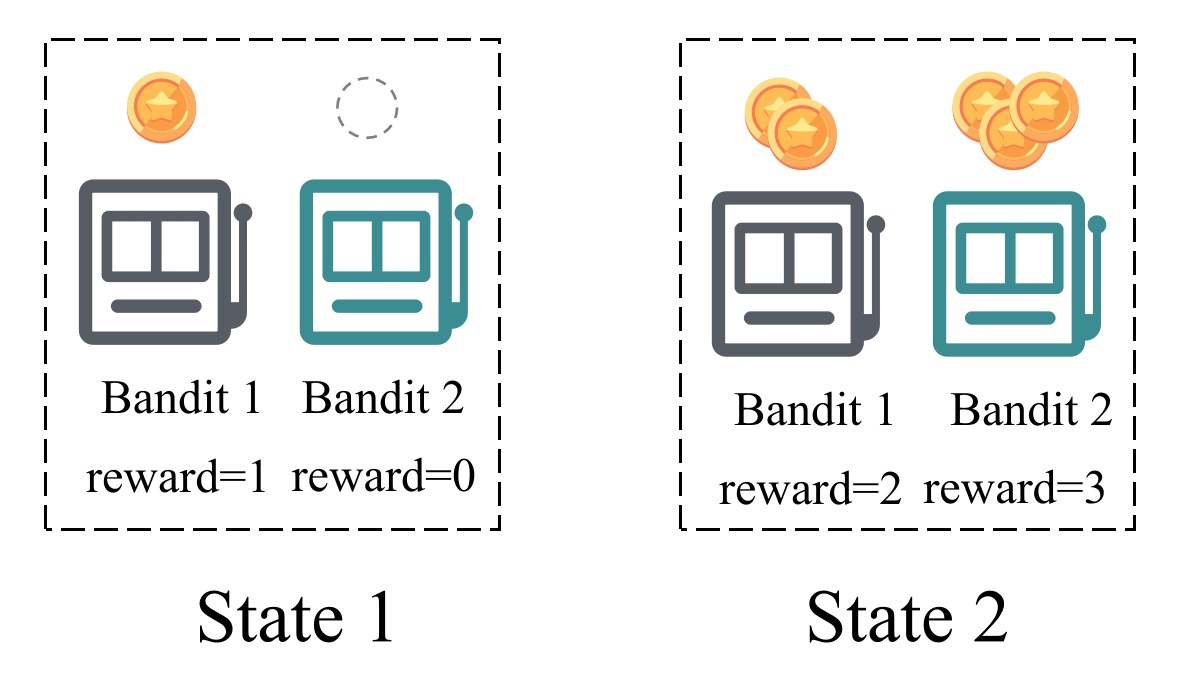
\includegraphics[width=.6\textwidth]{Figures/2024-fall-Bandit.png}
	\caption{Illustration of the two armed-bandit.}\label{fig:bandit}
\end{figure}


%\newpage
% \bibliography{refs}
%\bibliographystyle{abbrv}

%%%%%%%%%%%%%%%%%%%%%%%%%%%%%%%%%%%%%%%%%%%%%%%%%%%%%%%%%%%%%%%%

\end{document}
